%%% template.tex
%%%
%%% This LaTeX source document can be used as the basis for your technical
%%% paper or abstract.
%%%
%%% This example is tailored toward the two-page abstract. Please see "template.tex"
%%% for a more fully-annotated example.

\documentclass{acmsiggraph}

%%% Title of your article or abstract.

\title{This Is The Title of My Document}

\author{Stephen N. Spencer\thanks{e-mail:spencer@cs.washington.edu}\\Chair, ACM SIGGRAPH Publications Committee}
\pdfauthor{Stephen N. Spencer}

%%% Used by the ``review'' variation; the online ID will be printed on 
%%% every page of the content.

\TOGonlineid{45678}

% User-generated keywords.

\keywords{radiosity, global illumination, constant time}

% With the "\setcopyright" command the appropriate rights management text will be added
% to your document.

%\setcopyright{none}
%\setcopyright{acmcopyright}
%\setcopyright{acmlicensed}
\setcopyright{rightsretained}
%\setcopyright{usgov}
%\setcopyright{usgovmixed}
%\setcopyright{cagov}
%\setcopyright{cagovmixed}
%\setcopyright{rightsretained}

% The year of publication in the "\copyrightyear" command.

\copyrightyear{2016}

%%% Conference information, from the completed rights management form.
%%% The "\conferenceinfo" command has two parameters: 
%%%    - conference name
%%%    - conference date and location
%%% The "\isbn" field includes the year and month after the article ISBN.

\conferenceinfo{SIGGRAPH 2016 Posters}{July 24-28, 2016, Anaheim, CA} 
\isbn{978-1-4503-ABCD-E/16/07} 
\doi{http://doi.acm.org/10.1145/9999997.9999999}

\begin{document}

%%% This is the ``teaser'' command, which puts an figure, centered, below 
%%% the title and author information, and above the body of the content.

 \teaser{
   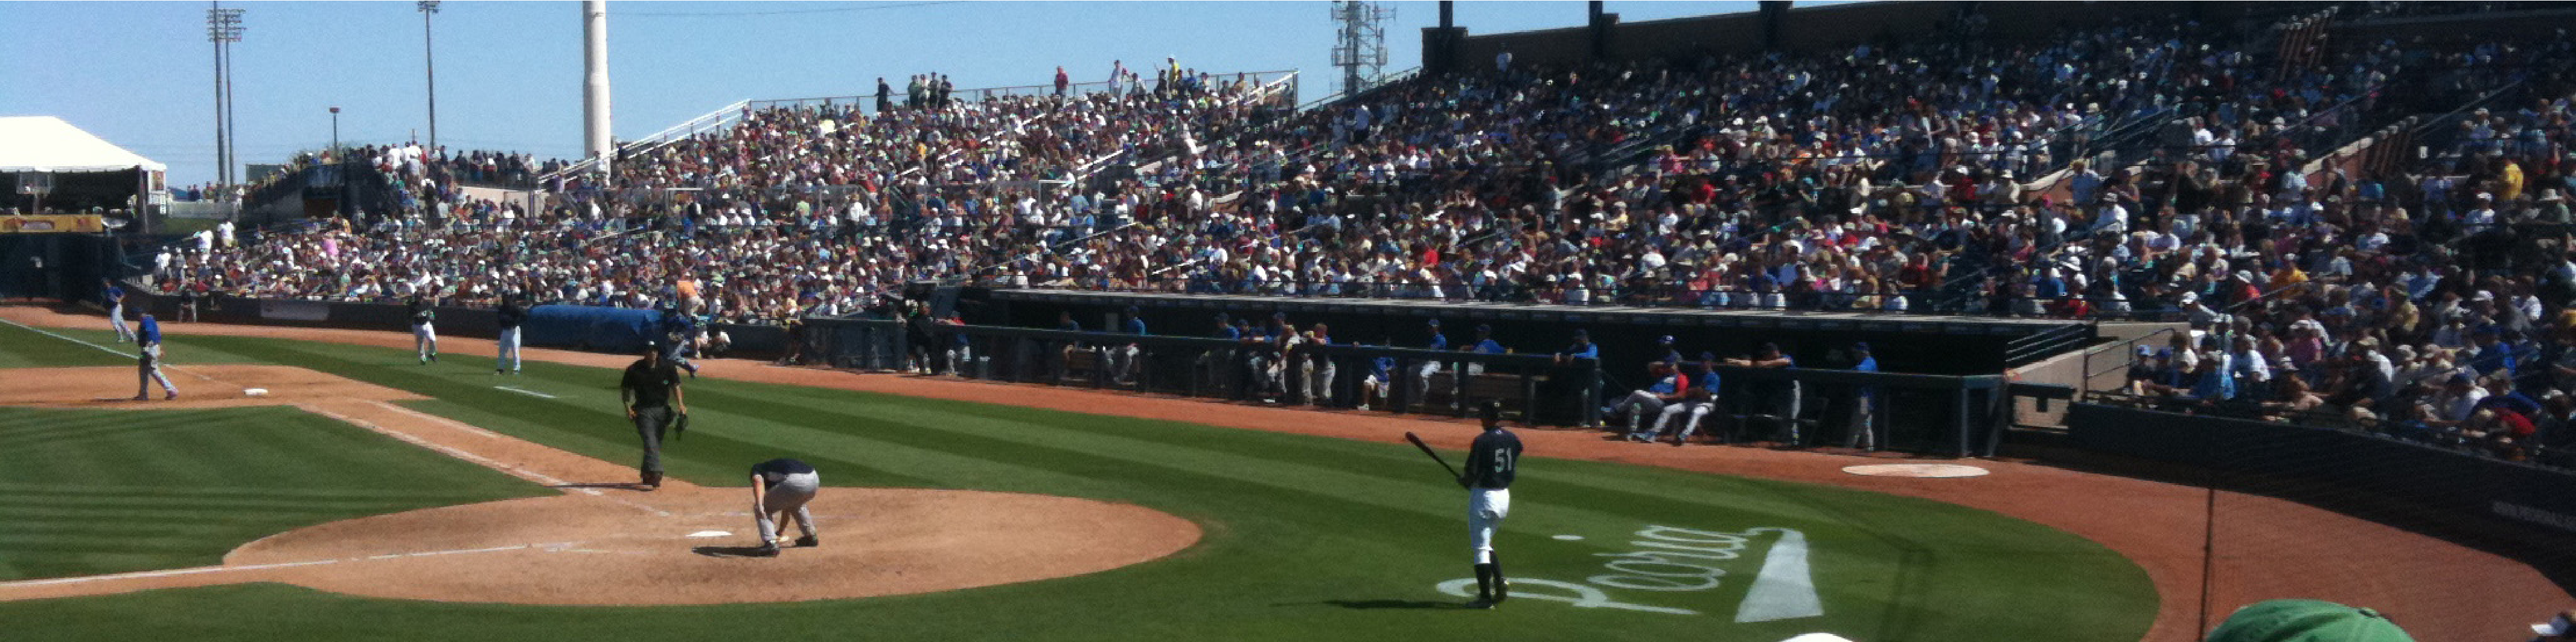
\includegraphics[height=1.5in]{images/sampleteaser}
   \caption{Spring Training 2009, Peoria, AZ.}
 }

\maketitle

\begin{abstract}

In this sample paper, we describe the formatting requirements for
content accepted to SIGGRAPH-sponsored events. The same format can be
used for content ranging from a one- or two-page Poster or Talk abstract, to a
full-length Technical Paper. 

[New for 2016] Authors are now responsible for adding the appropriate rights management
text to their final content, by adding information found on one's completed 
rights management form to the source document.

[New for 2016] Authors are now required to use ACM's current Computing Classification
System for the inclusion of appropriate subject concepts.

Please view the accompanying README file for a complete description of the formatting
specifications.

\end{abstract}

%
% The code below should be generated by the tool at
% http://dl.acm.org/ccs.cfm
% Please copy and paste the code instead of the example below. 
%
\begin{CCSXML}
<ccs2012>
<concept>
<concept_id>10010147.10010371.10010382</concept_id>
<concept_desc>Computing methodologies~Image manipulation</concept_desc>
<concept_significance>500</concept_significance>
</concept>
<concept>
<concept_id>10010147.10010371.10010382.10010236</concept_id>
<concept_desc>Computing methodologies~Computational photography</concept_desc>
<concept_significance>300</concept_significance>
</concept>
</ccs2012>
\end{CCSXML}

\ccsdesc[500]{Computing methodologies~Image manipulation}
\ccsdesc[300]{Computing methodologies~Computational photography}

%
% End generated code
%

% The next three commands are required, and insert the user-generated keywords, 
% The CCS concepts list, and the rights management text.
% Please make sure there is a blank line between each of these three commands.

\keywordlist

\conceptlist

\printcopyright

\section{First Section Heading}

Ut sagittis arcu ut turpis sodales, nec venenatis magna efficitur. Fusce non rhoncus risus, ac tincidunt arcu. Nulla lacus odio, accumsan tempor dolor sit amet, tincidunt porttitor justo. Quisque vulputate ex ac purus ultrices tristique. Pellentesque habitant morbi tristique senectus et netus et malesuada fames ac turpis egestas. Curabitur sed ullamcorper metus. Phasellus eu purus eget leo vulputate auctor vel scelerisque velit.

\begin{table}[ht]
  \centering
  \caption{A simple table.}
  \begin{tabular}{|r|l|}
    \hline
    7C0 & hexadecimal \\
    3700 & octal \\ \cline{2-2}
    11111000000 & binary \\
    \hline \hline
    1984 & decimal \\
    \hline
  \end{tabular}
\end{table}
  
Etiam sed mattis justo. Mauris lorem sapien, pellentesque vel viverra varius, porta ut nisi. Cras vel interdum dui, vitae fermentum elit. Nulla eu libero finibus, bibendum elit nec, ullamcorper velit. Donec ultrices, purus id ullamcorper euismod, ipsum erat sodales augue, ut sagittis sapien magna nec ex. Nulla massa arcu, suscipit non molestie ut, tristique id tellus. Maecenas nec malesuada mauris, vitae mattis sem. Quisque at risus quis arcu eleifend lacinia non sed neque.

\section{Second Section Heading}

Ut sagittis arcu ut turpis sodales, nec venenatis magna efficitur. Fusce non rhoncus risus, ac tincidunt arcu. Nulla lacus odio, accumsan tempor dolor sit amet, tincidunt porttitor justo. Quisque vulputate ex ac purus ultrices tristique. Pellentesque habitant morbi tristique senectus et netus et malesuada fames ac turpis egestas. Curabitur sed ullamcorper metus. Phasellus eu purus eget leo vulputate auctor vel scelerisque velit.

\subsection{This is a subsection}

Nunc vitae lorem nec diam ultrices fringilla. Aliquam volutpat metus ut magna bibendum, sed ultricies nunc placerat. Nulla volutpat rutrum vehicula. Cum sociis natoque penatibus et magnis dis parturient montes, nascetur ridiculus mus. Aliquam vel ligula elit. Nulla fermentum purus eu venenatis mollis. Nulla placerat dui accumsan urna pharetra maximus. Sed nec orci arcu. Suspendisse faucibus blandit libero ut feugiat. Nulla vitae imperdiet nulla. Cum sociis natoque penatibus et magnis dis parturient montes, nascetur ridiculus mus.

Etiam sed mattis justo. Mauris lorem sapien, pellentesque vel viverra varius, porta ut nisi. Cras vel interdum dui, vitae fermentum elit. Nulla eu libero finibus, bibendum elit nec, ullamcorper velit. Donec ultrices, purus id ullamcorper euismod, ipsum erat sodales augue, ut sagittis sapien magna nec ex. Nulla massa arcu, suscipit non molestie ut, tristique id tellus. Maecenas nec malesuada mauris, vitae mattis sem. Quisque at risus quis arcu eleifend lacinia non sed neque.

\subsection{This is another subsection}

Praesent lacinia, risus eget lacinia elementum, lorem elit ullamcorper arcu, quis condimentum ipsum dui at felis. Mauris maximus at lectus condimentum efficitur. Maecenas luctus, magna nec porttitor semper, justo libero semper nisi, nec commodo nunc turpis a velit. Morbi ac elementum urna, in elementum massa. Mauris ipsum turpis, fringilla in pellentesque a, mattis non erat. Cras vitae sodales lacus. Mauris sit amet laoreet ipsum. Maecenas quis consectetur dui. Nunc vulputate, dui eu blandit volutpat, augue dui molestie risus, et viverra lorem ligula quis eros.

\begin{figure}[ht]
  \centering
  \includegraphics[width=3.0in]{images/ferrari_laferrari}
  \caption{Ferrari LaFerrari. Image courtesy Flickr user ``gfreeman23.''}
  \label{fig:ferrari}
\end{figure}

\section{Third Section Heading}

Ut sagittis arcu ut turpis sodales, nec venenatis magna efficitur. Fusce non rhoncus risus, ac tincidunt arcu. Nulla lacus odio, accumsan tempor dolor sit amet, tincidunt porttitor justo. Quisque vulputate ex ac purus ultrices tristique. Pellentesque habitant morbi tristique senectus et netus et malesuada fames ac turpis egestas. Curabitur sed ullamcorper metus. Phasellus eu purus eget leo vulputate auctor vel scelerisque velit.

Nunc vitae lorem nec diam ultrices fringilla. Aliquam volutpat metus ut magna bibendum, sed ultricies nunc placerat. Nulla volutpat rutrum vehicula. Cum sociis natoque penatibus et magnis dis parturient montes, nascetur ridiculus mus. Aliquam vel ligula elit. Nulla fermentum purus eu venenatis mollis. Nulla placerat dui accumsan urna pharetra maximus. Sed nec orci arcu. Suspendisse faucibus blandit libero ut feugiat. Nulla vitae imperdiet nulla. Cum sociis natoque penatibus et magnis dis parturient montes, nascetur ridiculus mus.

Etiam sed mattis justo. Mauris lorem sapien, pellentesque vel viverra varius, porta ut nisi. Cras vel interdum dui, vitae fermentum elit. Nulla eu libero finibus, bibendum elit nec, ullamcorper velit. Donec ultrices, purus id ullamcorper euismod, ipsum erat sodales augue, ut sagittis sapien magna nec ex. Nulla massa arcu, suscipit non molestie ut, tristique id tellus. Maecenas nec malesuada mauris, vitae mattis sem. Quisque at risus quis arcu eleifend lacinia non sed neque.

\section*{Acknowledgements}

To Robert, for all the bagels.

\bibliographystyle{acmsiggraph}
\nocite{*}
\bibliography{template}
\end{document}
